\documentclass[UTF8,zihao=-4]{ctexart}
\usepackage{graphicx}
\usepackage{geometry}
\usepackage{siunitx}
\usepackage{amsmath}
\usepackage{amsfonts}
\usepackage{amssymb}
\usepackage{listings}
\usepackage{forest}
\usepackage{tikz}
\lstset{
	language=SQL,
	breaklines,
	tabsize=4,
	basicstyle=\ttfamily \small,
	showstringspaces=false
}
\geometry{a4paper,centering,scale=0.8}
\title{\heiti 数据库\quad 第一次实验}
\author{PB17000005\quad \CJKfontspec{AR PL UKai CN} 赵作竑}
\date{\kaishu \today}
\begin{document}
	\maketitle
	\begin{enumerate}
		\item[1] 首先创建数据库:
		\begin{lstlisting}
create database if not exists Lab1 default character set utf8mb4 collate utf8mb4_general_ci;
use Lab1;
		\end{lstlisting} 
		接下来创建三个基本表:
		\begin{lstlisting}
create table book (
  id char(8) primary key,
  name varchar(50) not null,
  author varchar(50),
  price float unsigned,
  status enum('0', '1') default '0'
);
create table reader (
  id char(10) primary key,
  name varchar(10),
  age int unsigned,
  address varchar(20)
);
create table borrow (
  book_id char(8),
  reader_id char(10),
  borrow_date date,
  return_date date,
  primary key (book_id, reader_id, borrow_date),
  foreign key (book_id) references book(id),
  foreign key (reader_id) references reader(id)
);
		\end{lstlisting} 
		\item[2] 先来看实体完整性。比如,我们插入两本主键重复(也就是\texttt{id}相同)的书:
		\begin{lstlisting}
insert into book value (
    "80029089",
    "Learning MySQL",
    "Williams",
    90.83,
    '0'
  );
insert into book value (
    "80029089",
    "Learning MySQL2",
    "Williams",
    90.83,
    '0'
  );
		\end{lstlisting} 
		会得到错误信息:\texttt{(1062, "Duplicate entry '80029089' for key 'PRIMARY'")}。
		
		接着来看参照完整性。假如我们插入一条借阅记录:
		\begin{lstlisting}
insert into borrow value (
    "00511407",
    "PB17000005",
    "2020-03-10",
    NULL
  );
		\end{lstlisting}
		而book表中并没有关于\texttt{id="00511407"}的书,那么此时会有错误提示:
		\begin{lstlisting}
(1452, 'Cannot add or update a child row: a foreign key constraint fails (`Lab1`.`borrow`, CONSTRAINT `borrow_ibfk_1` FOREIGN KEY (`book_id`) REFERENCES `book` (`id`))')
		\end{lstlisting}

		最后我们来看用户自定义完整性。我们知道,每本书的状态要么是已借出,要么是没有借出,分别用1和0表示。
		如果我们试图录入一条书籍信息,并且它的状态并不是0或1:
		\begin{lstlisting}
insert into book value (
    "00511407",
    "编译程序设计理论",
    "刘易斯",
    44.44,
    5
  );
		\end{lstlisting}
		会得到错误:\texttt{(1265, "Data truncated for column 'status' at row 1")}。
		\item[3(1)] 检索读者``{\CJKfontspec{AR PL UMing CN} 赵作竑}''的读者号和地址:
		\begin{center}
			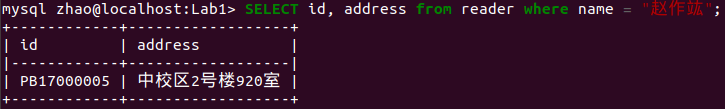
\includegraphics[width=\linewidth]{3-1.png}
		\end{center} 
		\item[3(2)] 检索读者``{\CJKfontspec{AR PL UMing CN} 赵作竑}''所借阅的书(包括已还和未还图书)的图书名和借期;
		\begin{center}
			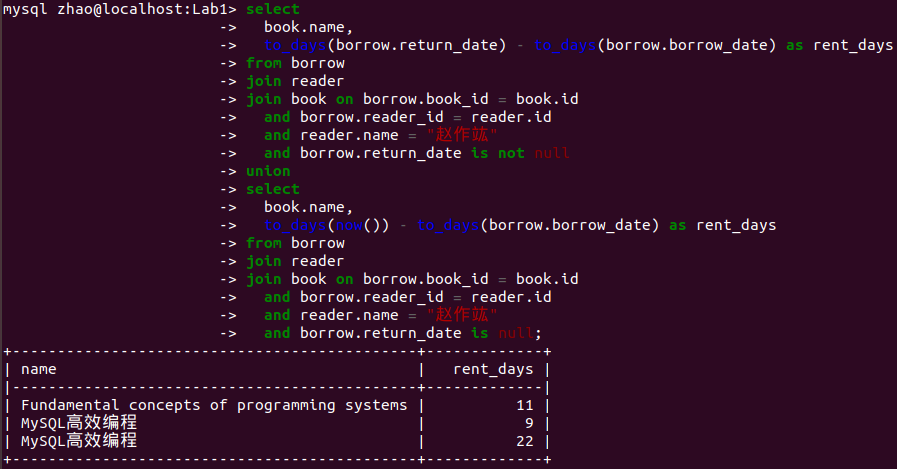
\includegraphics[width=\linewidth]{3-2.png}
		\end{center}
		``借期''的计算方式是:如果这本书已经归还,则是从开始借阅到归还的天数;如果这本书还没有归还,则租期是从开始借阅到现在的天数。

		注意,这里《MySQL高效编程》出现了两次,原因是在我设计的测试数据中,我一共借了这本书两次。
		\item[3(3)] 检索未借阅图书的读者(当前):
		
		首先,我们要找出现在还在借阅图书的读者,之后我们从全部读者的列表中去掉这些读者,就得到了当前没有借阅图书的读者。
		\begin{center}
			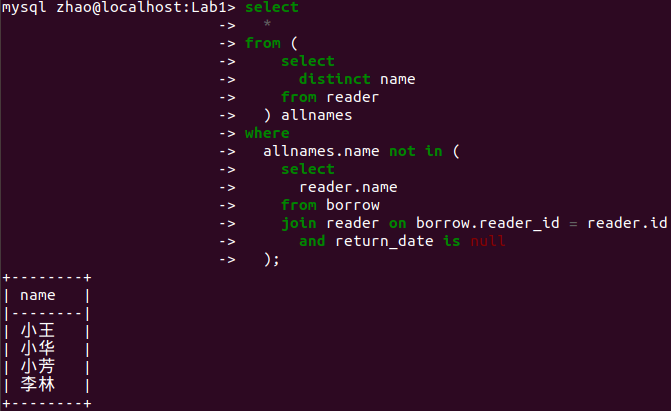
\includegraphics[width=\linewidth]{3-3.png}
		\end{center} 
		\item[3(4)] 检索Ullman所写的书的书名和单价:
		\begin{center}
			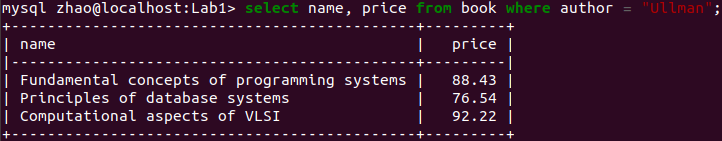
\includegraphics[width=\linewidth]{3-4.png}
		\end{center} 
		\item[3(5)] 检索读者``李林''借阅未还的图书的图书号和书名;
		\begin{center}
			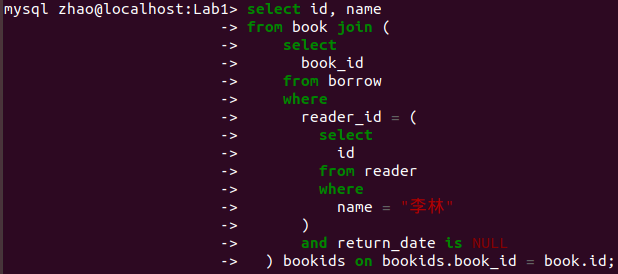
\includegraphics[width=\linewidth]{3-5.png}
		\end{center} 
		由于测试数据的原因,结果为空。
		\item[3(6)] 检索借阅图书数目超过3本的读者姓名(建馆以来):
		\begin{center}
			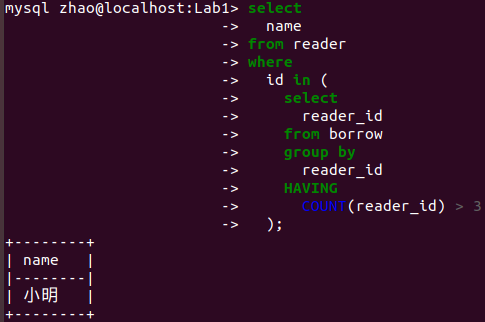
\includegraphics[width=0.85\linewidth]{3-6.png}
		\end{center} 
		\item[3(7)] 检索没有借阅读者``李林''所借的任何一本书的读者姓名和读者号(建馆以来);
		\begin{center}
			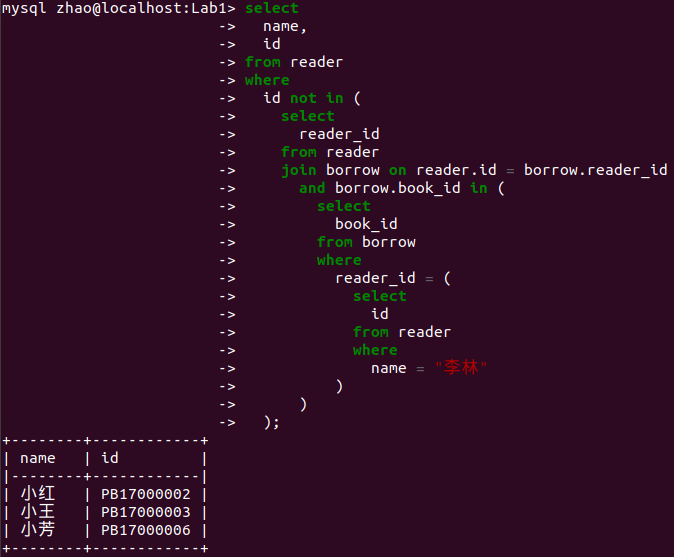
\includegraphics[width=0.85\linewidth]{3-7.png}
		\end{center} 
		\item[3(8)] 检索书名中包含``MySQL''的图书书名及图书号(不区分大小写);
		\begin{center}
			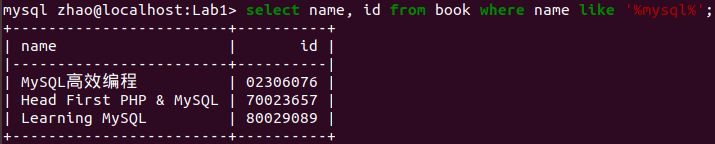
\includegraphics[width=\linewidth]{3-8.png}
		\end{center} 
		\item[3(9)] 创建一个读者借书信息的视图,该视图包含读者号、姓名、所借图书号、图书名和借期;
		并使用该视图查询最近一年所有读者的读者号以及所借阅的不同图书数(重复借阅仍计入计数)。 
		\begin{center}
			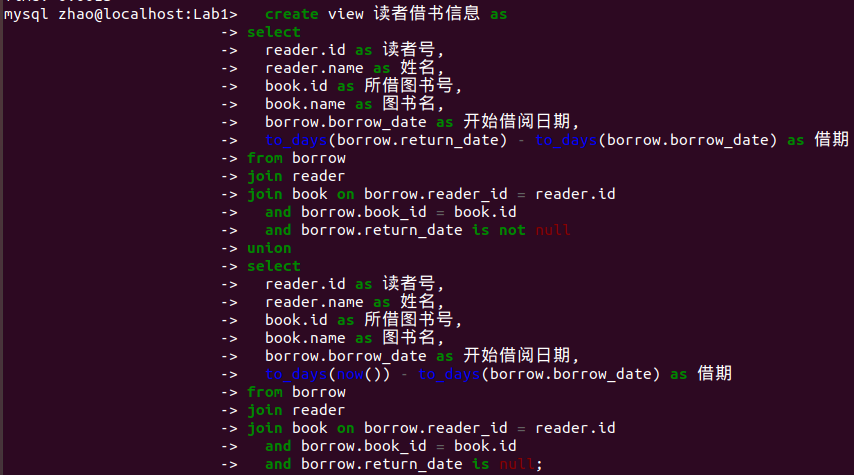
\includegraphics[width=\linewidth]{3-9-1.png}

			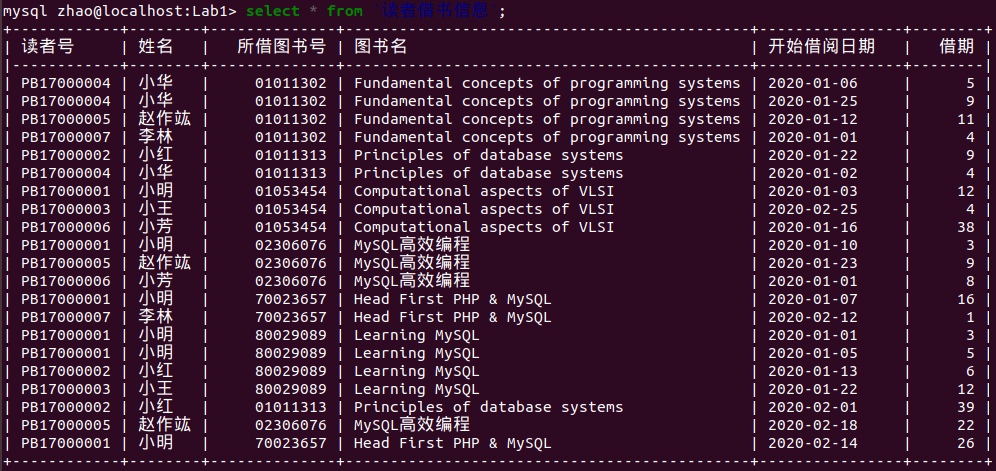
\includegraphics[width=\linewidth]{3-9-2.png}
		\end{center} 
		接下来我们用该视图进行查询:
		\begin{center}
			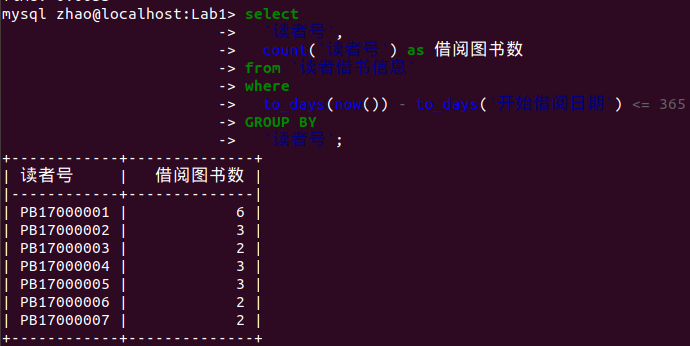
\includegraphics[width=\linewidth]{3-9-3.png}
		\end{center}
	\end{enumerate}
\end{document}